\section{系统开发成果}

对西安石油大学计算机学院 GMS 系统进行的第二期工程已完成设计与开发,通过测试并于 2018 年 5 月运行在西安石油大学内,校园网网址:\underline{http://bkbysj.xsyu.edu.cn/}。将承接计算机学院 2018 年毕业生毕业设计相关线上工作。

\subsection{毕业设计答辩模块}

整个毕业设计答辩阶段的流程从管理员划分答辩小组开始,该划分操作逻辑复杂,既要考虑组内教师的职称、工作年限,又要综合考虑教师今年所指导的学生(尽量使学生的指导教师不在其答辩组内)。所以,系统将划分答辩小组的操作交由管理员进行,线上系统则提供辅助决策的作用。

管理员在如图 \ref{divide-show} 所示的页面中进行答辩小组划分。首先下载一个由系统生成的 Excel 文档,该文档中包含由答辩系统预生成的小组划分表。然后以该表作为参考,管理员对小组划分进行微调,完成后将该表回传至系统内,即可完成当年的答辩小组划分。

\begin{figure}
	\centering
	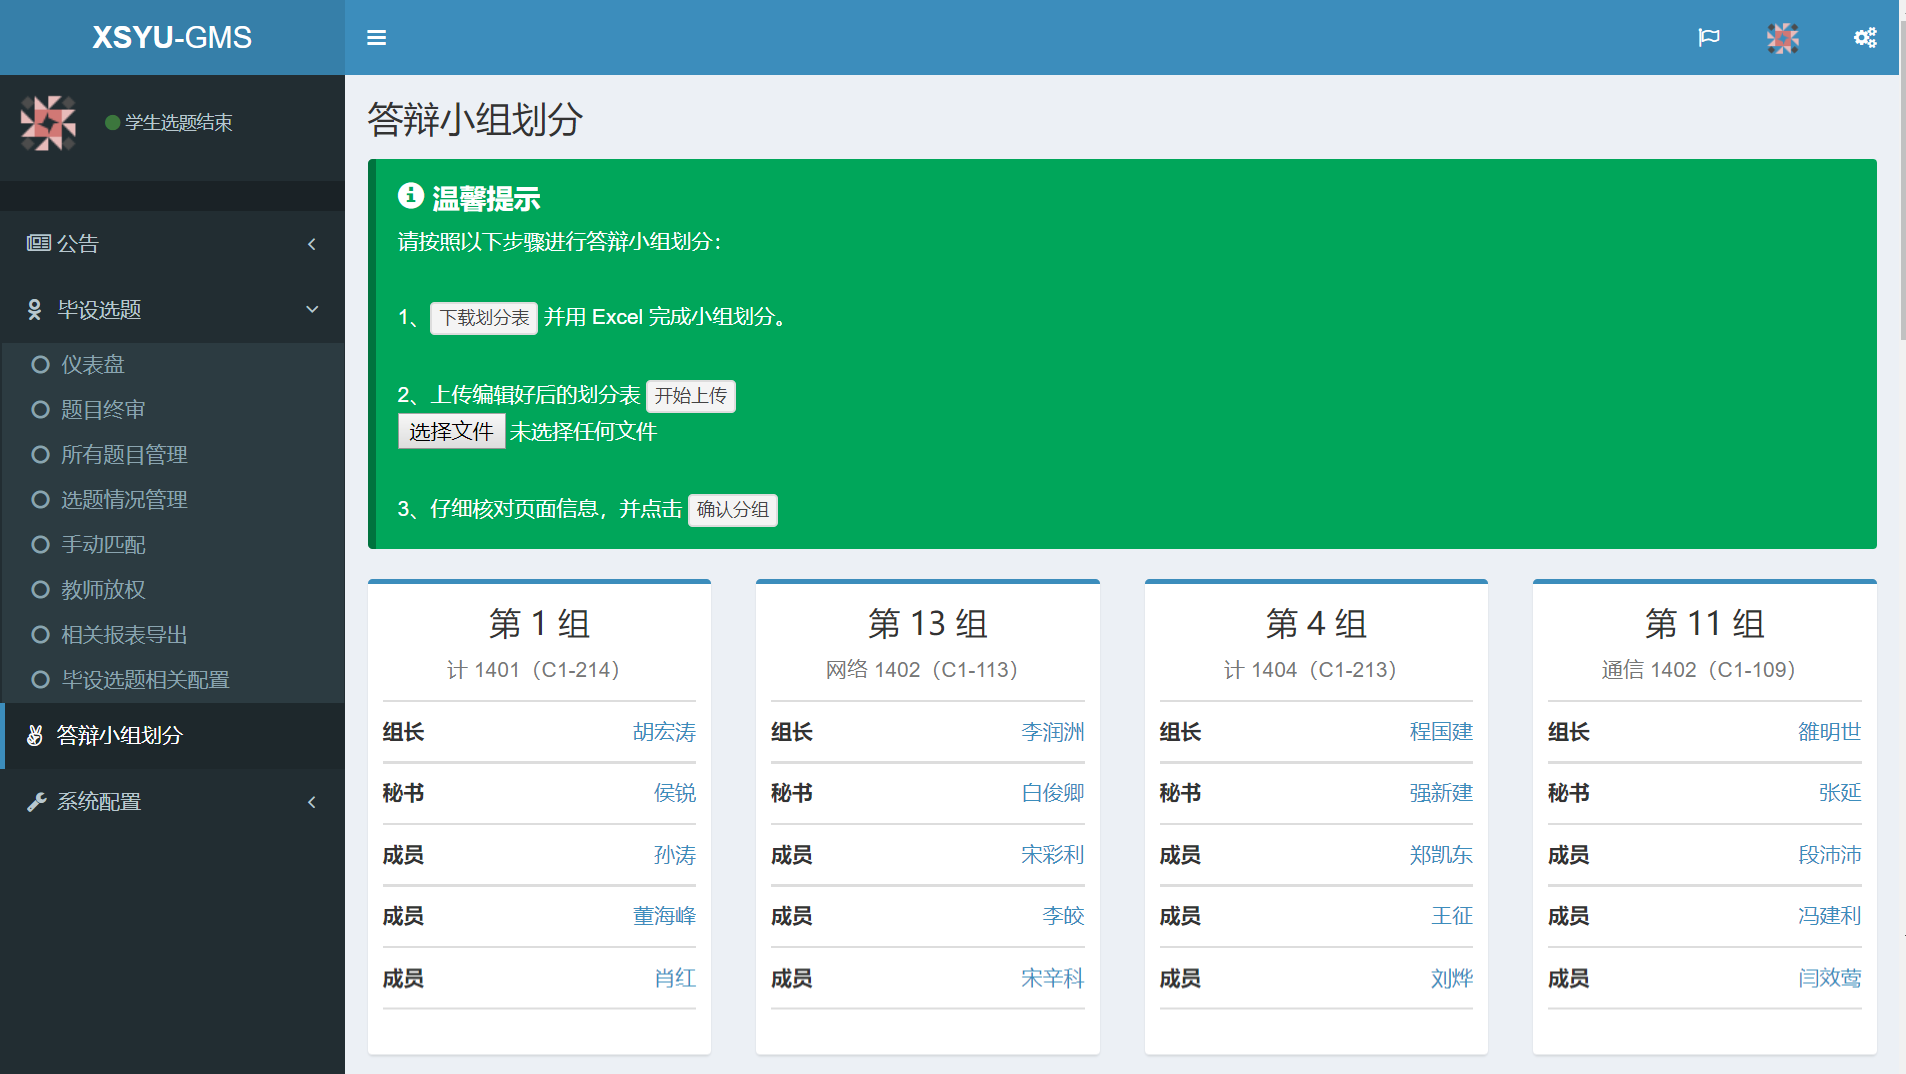
\includegraphics[width=1\linewidth]{figure/divide-show}
	\caption{管理员答辩小组划分页面}
	\label{divide-show}
\end{figure}

在管理员完成答辩小组划分之后的下一个流程,是指导教师对自己所带学生进行论文审阅。进入图 \ref{tealook} 所示页面后,依次对学生们点击“进行论文审阅”按钮,输入分数和内容即可完成审阅操作,并下载论文审阅书。这时该学生的“进行论文审阅”按钮会变成“√修改论文审阅”,再次点击该按钮可对已审阅的内容进行修改。

该页面同时是每位教师对自己所带学生的管理页面(关键信息已模糊化处理)。值得一说的是,本系统中所有的用户头像均不相同,根据用户 UID 哈希生成的随机矢量风格,避免了所有老师学生都使用默认头像的尴尬又无聊的景象。

\begin{figure}
	\centering
	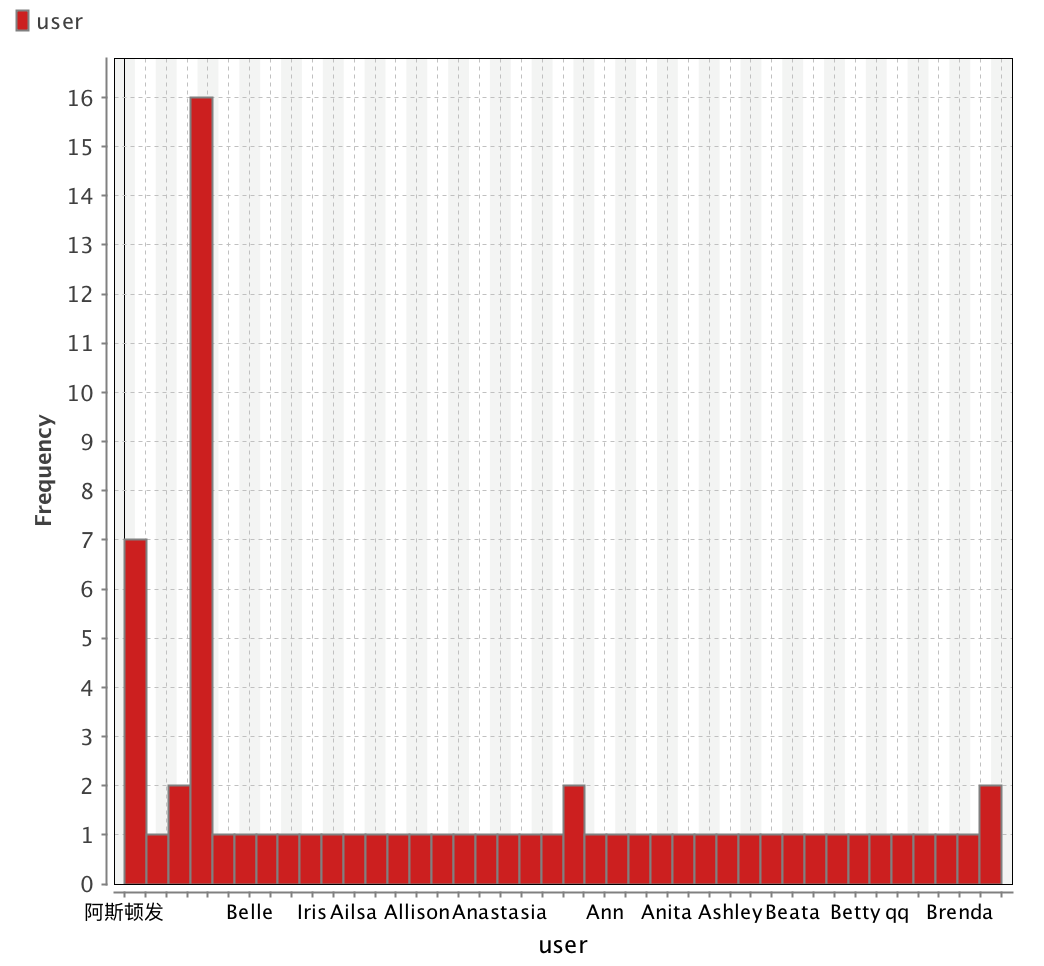
\includegraphics[width=\linewidth]{figure/5-1}
	\caption{教师管理所带学生页面}
	\label{tealook}
\end{figure}

审阅阶段过后,答辩流程将会进入到评阅环节,教师进行答辩评阅的页面如图 \ref{tea-review} 所示。添加评阅时,教师在线下阅读学生的论文及相关资料,然后在系统中输入该学生的学号、评阅内容、评阅成绩,即可完成评阅操作。为了方便教师操作,可支持仅输入学号后数位,系统会自动匹配到对应学生并完成评阅操作,如果存在相同学号后缀的学生,系统亦会给与提示。

从截图中可以看出,系统同时显示出了教师所属的班级,以及小组的答辩地点,这是在深度了解教师需求后开发的人性化功能。评阅教师在完成所有评阅数据的录入后,可点击“生成评阅意见表”按钮,会下载得到一个压缩包,内包含评阅的所有学生各自的评阅意见表,该表符合学校相关的格式要求,可直接提供给学校教务处。

\begin{figure}
	\centering
	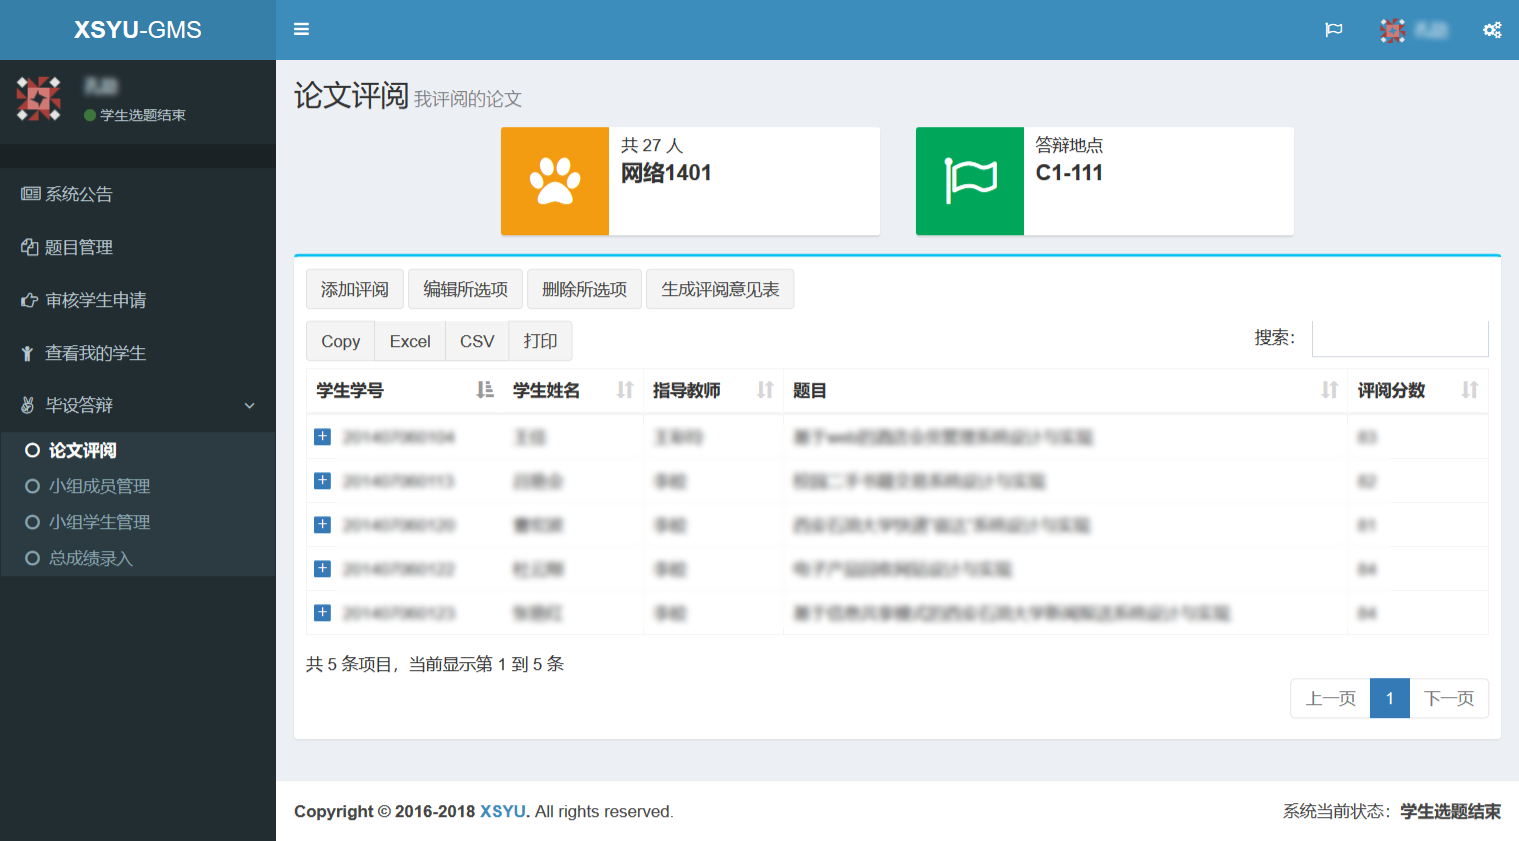
\includegraphics[width=\linewidth]{figure/tea-review}
	\caption{答辩组成员评阅页面}
	\label{tea-review}
\end{figure}

在此系统中小组秘书拥有最多的线上功能,包括统计组内成员工作量以供生成工作量统计表,以及小组内学生的答辩成绩、总成绩的录入。秘书的成绩录入工作使用 Excel 辅助进行,而非在网页上逐次添加。秘书首先下载一个系统自动生成的小组内学生名单,其中包括学生的审阅成绩和评阅成绩。只需要输入答辩成绩之后,总成绩会自动按照公式生成。最后再将填写完成后的 Excel 文档上传,即可完成组内学生成绩的录入。

完成答辩阶段所有数据的录入之后,管理员和答辩秘书、答辩组长同时拥有类似图 \ref{data-show} 的数据展示页面,以表格的形式展现出对应权限所拥有的学生、题目等数据和信息,表格也可以很方便的自定义按列排序、搜索关键字,以及导出为 Excel、PDF 等格式。

\begin{figure}
	\centering
	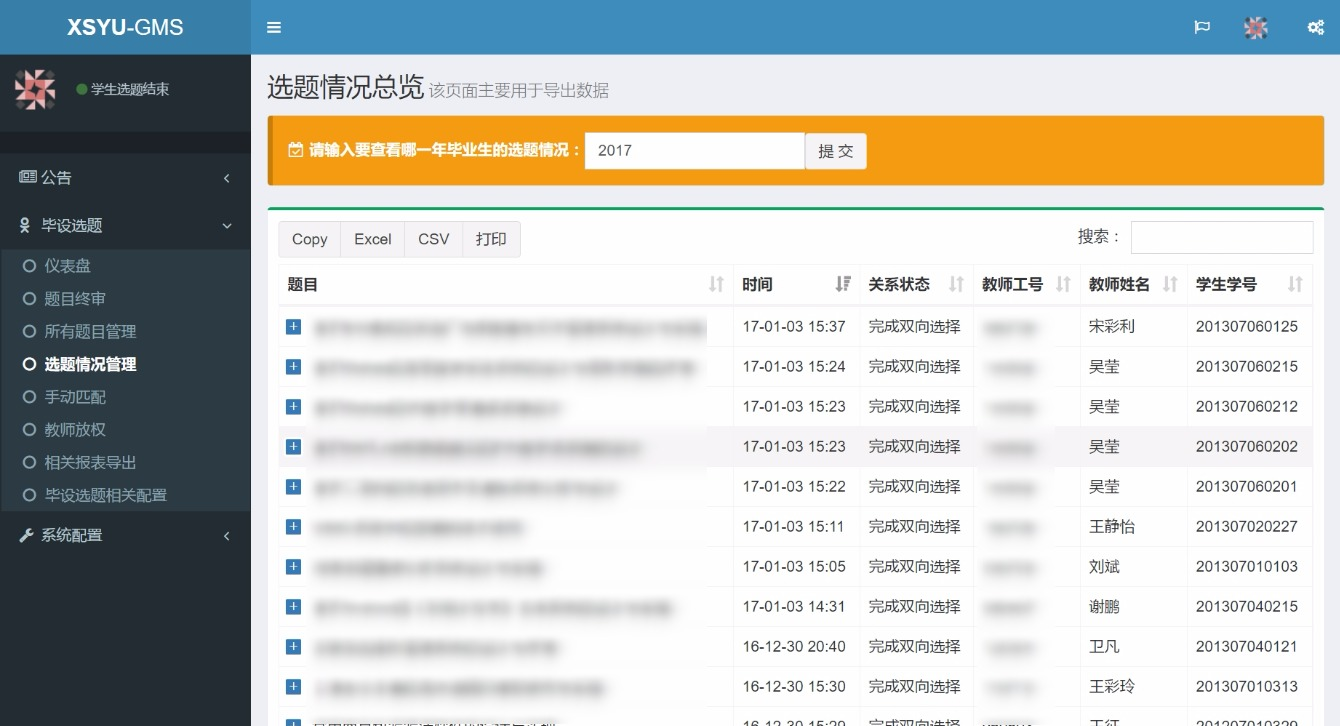
\includegraphics[width=\linewidth]{figure/5-3}
	\caption{答辩相关数据展示页面}
	\label{data-show}
\end{figure}


\subsection{系统内其他辅助模块}

专门为管理员设计的功能占整个系统工作量的 60\% 以上。在管理员面板中,可以管理所有的用户,设定每位用户的类型,也可以看到现在所有选题配对情况。值得一说的是,管理员支持使用 Excel 批量导入每届学生老师信息,系统会自动解析 xlsx 文档,并创建对应的登陆账号。此外,本系统网页中所有可见的表格信息均可一键导出为 Excel 或 Word 文档,方便进一步办公处理。

图 \ref{admin-panel} 是管理员对全院学生综合管理的仪表盘页面,在这里利用了数据可视化技术,将全院所有学生的综合情况清晰地展现在管理员面前。在这里,可以直观的看到待选题目和学生总数的柱状对比图,也可以分专业以饼状图的形式看到当前各专业学生的选题状态分布。这些都是选题流程中管理员需要掌握的数据。

\begin{figure}
	\centering
	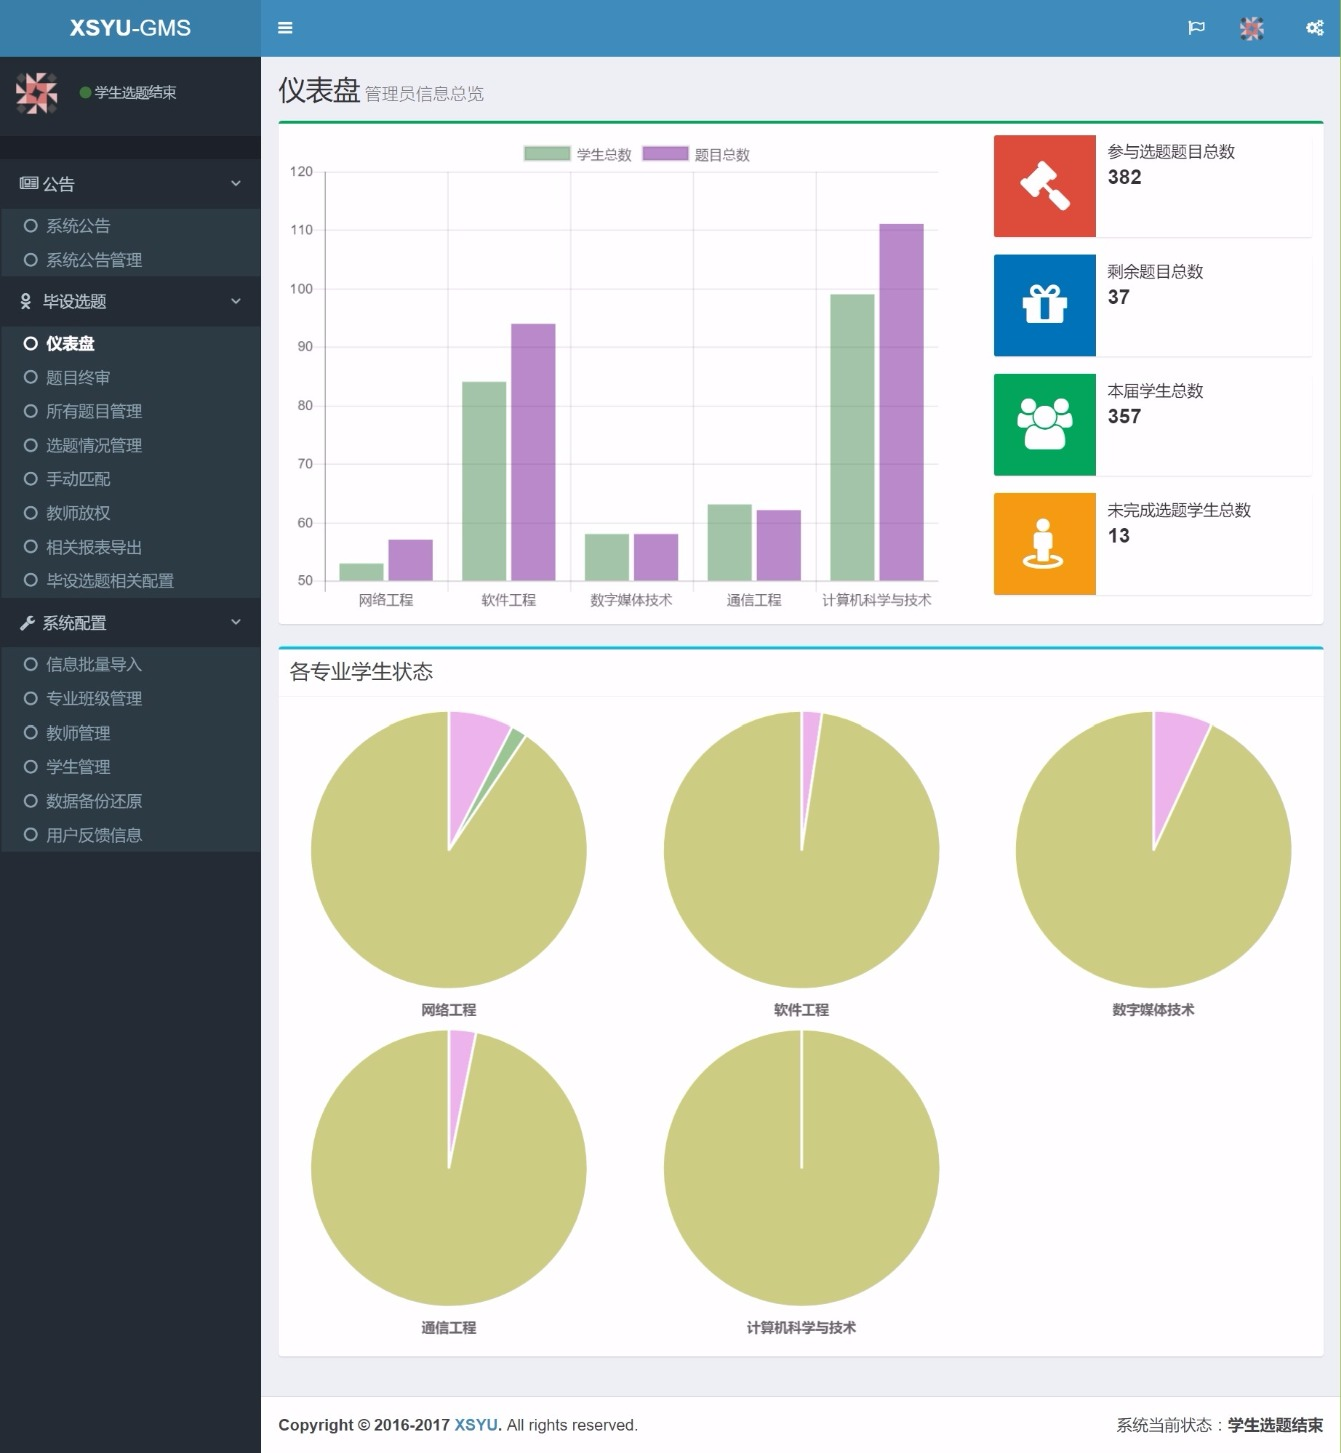
\includegraphics[width=0.85\linewidth]{figure/5-2}
	\caption{管理员仪表盘页面}
	\label{admin-panel}
\end{figure}

学生作为本系统中最简单的角色,可进行选题,以及在选题成功之后通过此系统向老师发送文件。在选题方面设计了 2 个人性化的特性:能看到某道题当前已选人数,这大大避免某道题被大家集中选择;在教师查看你的选题志愿之前,可以取消申请,并另选一道题。(事实上在此系统中所有的状态转移均支持最大程度的撤销操作)

该系统中的教师角色可以出题,并且实时跟踪自己题目的状态,历年所出题目会形成一个自己的题库以供复用,题目支持上传附件。这些特性弥补了计算机学院旧选题系统的遗憾。

本系统还拥有一个强大的自动备份还原功能,系统会自动在每天凌晨 3 时进行一次数据库备份,同时自动删除 15 天前的备份(不支持手动删除),当然,用户可以选择在需要的时候随时手动创建一个备份。这样的设计使得系统更加稳定,无论是管理员的误操作,还是被任何形式的恶意攻击,都不会对系统造成很大的影响。

此外,如图 \ref{gms-news} 所示,本系统拥有完善的公告系统,支持富文本编辑、设置置顶、支持设置公告对不同类型用户的可见性,以及附件支持。

\begin{figure}
	\centering
	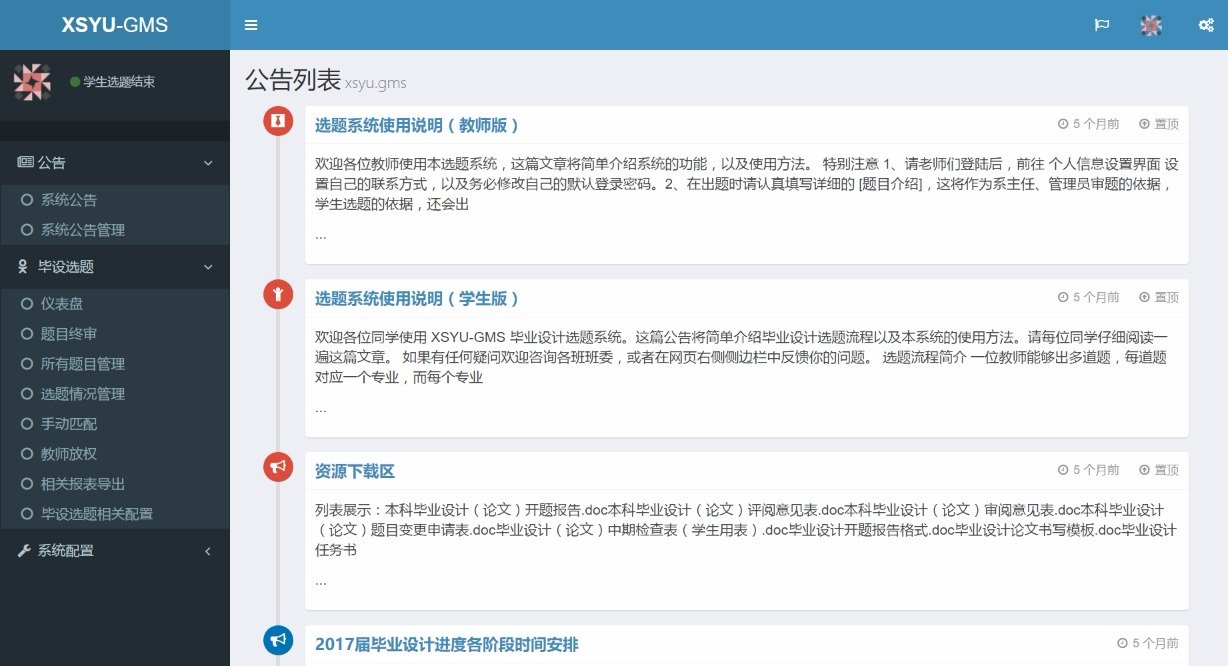
\includegraphics[width=1\linewidth]{figure/gms-news}
	\caption{GMS 公告系统}
	\label{gms-news}
\end{figure}
